\chapter{Fundamentos básicos}

Este capitulo apresenta os principais conceitos e definições necessários para o entendimento deste trabalho. A seção 2.1 apresenta alguns conceitos básicos em~\emph{Unified Modeling Language} (UML), que são necessários para o entendimento da modelagem deste trabalho.
A seção 2.2 disserta sobre conceitos a respeito da informática na educação.
A seção 2.3 aborda a teoria sobre Sistemas Multiagentes necessária para este trabalho.
A seção 2.4 contém a metodologia~\emph{Multiagent System Engineering}, desenvolvida para a criação de Sistemas Multiagentes
A seção 2.5 e 2.6 abordam o funcionamento dos frameworks JADE e Jboss Seam, respectivamente.
Por fim, a seção 2.7 detalha alguns trabalhos correlatos.

\section{Unified Modeling Language}

A Linguagem Unificada de Modelagem,~\emph{Unified Modeling Language} (UML) é uma linguagem visual que foi desenvolvida para a representação do software por meio de imagens, objetivando o entendimento dos artefatos de forma rápida e clara e resultando em uma semântica para o projeto em questão. De acordo com~\cite{fowler04} o UML faz parte de uma família de notações gráficas que ajudam na descrição e concepção de sistemas de software, principalmente em sistemas concebidos utilizando o paradigma da orientação à objetos (OO).

O UML é um padrão não proprietário, controlado pelo consórcio~\emph{Object Management Group}~\cite{omg20}. Seu nascimento é datado em 1997~\cite{fowler04}, surgindo a partir da união de diversas linguagens e ferramentas de surgiram na década de 80 e 90.
A linguagem ajuda o entendimento de como o software foi projetado, como ocorre a comunicação entre seus objetos, como suas classes são organizadas, quais são os atores que são envolvidos na utilização do software, dentre outras possibilidades de representação.

Em~\cite{fowler04}, é possível separar o uso do UML de três formas distintas, diferindo entre as modelagens utilizadas e o objetivo de uso. As três formas são: Rascunho, planta de software e como linguagem de programação. 

A utilização como rascunho é utilizada para facilitar a comunicação entre as pessoas envolvidas no projeto, sejam desenvolvedores discutindo funcionalidades do software ou gestores explicando funcionalidades em alto nível. O objetivo neste uso é a comunicação de alguns aspectos do sistema de forma rápida, sem a necessidade de formalizar artefatos para o projeto.

A utilização do UML como planta de software são documentos detalhados que são criados para documentação do software, sendo divida em duas sub-categorias: Engenharia reversa e engenharia avante. Na engenharia reversa, os diagramas são gerados a partir de uma ferramenta que faz a leitura do código fonte e gera os diagramas desejados, que são utilizados para auxiliar o leitor no entendimento do sistema. Na engenharia avante, a idéia é modelar o sistema detalhadamente antes de qualquer desenvolvimento, prevendo quais serão os módulos do sistema, bem como a sua a comunicação.

No uso como linguagem de programação, o UML é utilizado para geração de código executável por ferramentas avançadas de modelagem. Esse modo requer a modelagem de estado e comportamento do sistema, para fins de detalhar todo o comportamento e lógica do sistema em código.

\subsection{Diagramas UML}

O UML 2 descreve 13 tipos de diagramas que podem ser categorizados por estruturais e comportamentais. A imagem~\ref{fig:categorias-diagramas} ilustra essa categorização de diagramas.

\begin{figure}
	\centering
	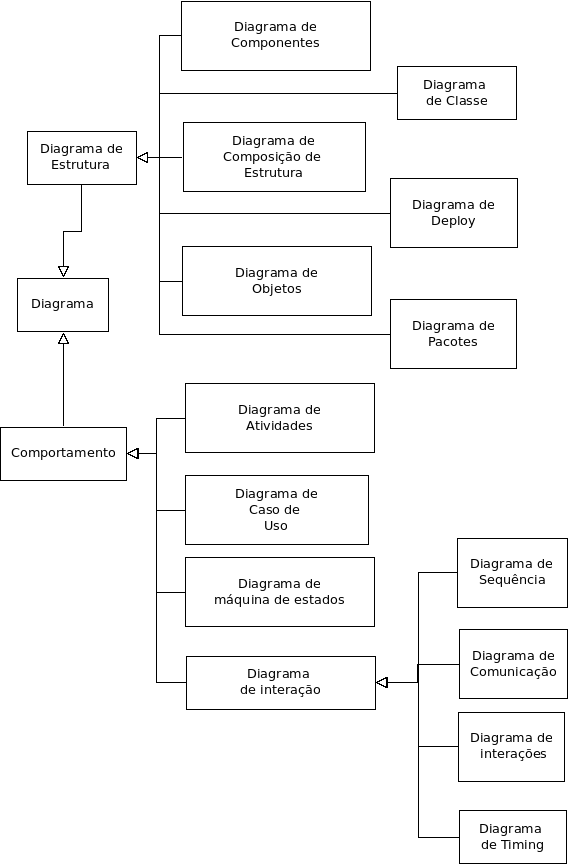
\includegraphics[scale=0.75]{images/categorias-diagramas.png}
	\caption{Diagramas categorizados por Estrutura e Comportamento. Fonte~\cite{fowler04}.}
	\label{fig:categorias-diagramas}
\end{figure}

Apesar da grande quantidade diagramas envolvidos no UML, nem todos os processos de desenvolvimentos de software utilizam todos eles. A maioria das pessoas utiliza-se de um conjunto de poucos diagramas para modelagem do sistema. Nas próximas subseções, serão detalhados apenas os seguintes diagramas, que são necessários para o entendimento deste trabalho:

\begin{itemize}
	\item Diagrama de Caso de uso
	\item Diagrama de sequência
\end{itemize}

\subsubsection{Diagrama de Caso de Uso}
Casos de uso são relatos textuais que são utilizados para descobrir e descrever os requisitos do sistema. Consiste da descrição de como um ator utiliza uma funcionalidade do sistema para atingir algum objetivo relacionado. De acordo com~\cite{larman08}, os casos de uso devem ser prioritariamente desenvolvidos de forma textual e o seu respectivo diagrama deve ser desenvolvido de forma secundária, somente para ilustrar o relato textual.

Um dos objetivos do caso de uso é a facilidade do levantamento dos requisitos, tanto para os analistas de um sistema, quanto para os clientes envolvidos. A definição de uma modelagem em comum facilidade entre as partes faz do caso de uso uma boa maneira de simplificar o entendimento do comportamento do sistema~\cite{larman08}, bem como envolver todos as partes interessadas do sistema(~\emph{stakeholders}) na construção do mesmo. De acordo com~\cite{cockburn01}, o caso de uso é um contrato de como será o comportamento do sistema. Este contrato será feito por meio dos atores que existirão, da sua interação com o sistema, bem como os cenários existentes.

Duas definições fazem-se necessárias para o entendimento do caso de uso. A primeira delas é o "Ator" do caso de uso. Ele é um objeto com um comportamento definido no sistema. É possível definir o ator como uma pessoa, organização ou mesmo o próprio sistema (quando utiliza serviços do próprio sistema), desde que tenham sempre um papel relacionado. Existem três tipos de atores relacionados ao sistema:
\begin{itemize}
	\item Ator Principal: Seus objetivos são satisfeitos por meio da utilização do sistema.
	\item Ator de Suporte: Fornece algum serviço para o sistema.
	\item Ator de Bastidor: Expressa algum interesse pelo comportamento do caso de uso.
\end{itemize}

A segunda definição envolvida é a de cenário. Um cenário é uma sequência de interações entre os atores e o sistema. Os cenários são separados por ações de interesses de atores. Logo o caso de uso pode ser considerado como um conjunto de cenários de interações de atores com o sistema.

Dessa forma, o caso de uso deve deixar claro os requisitos funcionais do sistema, bem como o seu comportamento. Existem três formas de se escrever um caso de uso, diferindo em seu nível de formalidade e formatos: Resumido, informal e completo. Este trabalho usará o nível de caso de uso completo, devido ao fato de ser estruturado e mostrar mais detalhes. Os casos de uso são estruturados de diversas formas de acordo com a literatura, sendo a mais famosa~\cite{larman08} a estrutura utilizada por Alistar Cockburn~\cite{cockburn01} e detalhada na tabela~\ref{tabela:topicos_uc}

\begin{table}
	\caption{Estruturação Detalhada de Caso de Uso}
	\begin{tabular}{|p{5cm} | p{9cm}|}
		\hline
		\textbf{Seção do Caso de Uso}	& \textbf{Significado} \\
		\hline
		Nome do Caso de Uso 	& Nome do caso de uso, iniciando-se com um verbo  \\
		\hline
		Escopo	& Escopo descrito pelo caso de uso \\
		\hline
		Nível	& Podem ser níveis de objetivo de usuário (quando descrevem os cenários para atingir o objetivo do usuário) ou nível de subfunção (subpassos para dar suporte a um objetivo de usuário) \\
		\hline
		Ator Principal	& O ator que procura os serviços para atingir seus objetivos  \\
		\hline
		Interessados e Interesses	& Significado  \\
		\hline
		Pré-Condições	& Condições que antecedem o caso de uso e são necessárias para atingir os objetivos \\
		\hline
		Garantia de Sucesso	& Objetos que podem ser analisados após a execução do caso de uso a fim de validar a correta execução do sistema  \\
		\hline
		Cenário de Sucesso Principal	& Chamado também de fluxo básico, este cenário descreve o fluxo principal do sistema que satisfaz os interesses dos interessados.  \\
		\hline
		Extensões	& Chamado também de fluxos alternativos, são fluxos auxiliares ou cenários de erros que são relacionados ao cenário de sucesso principal \\
		\hline
		Requisitos Especiais	& Registram requisitos não funcionais do sistema e que estão relacionados com o caso de uso \\
		\hline
		Lista de Variantes Tecnologias de Dados	& Listagem de dificuldades técnicas, desafios técnicos que valem a pena registrar no caso de uso \\
		\hline
		Frequência de ocorrência	& Frequência de ocorrência deste caso de uso \\
		\hline
	\end{tabular}
	\label{tabela:topicos_uc}
\end{table}

A diagramação do caso de uso por UML é uma forma de representação do sistema, mostrando fronteiras do sistema, comunicação e comportamento entre os atores. A figura~\ref{fig:diagrama-uml} mostra a sugestão de diagramação do caso de uso, propondo forma de representação de atores, casos de uso e atores auxiliares.

\begin{figure}
	\centering
	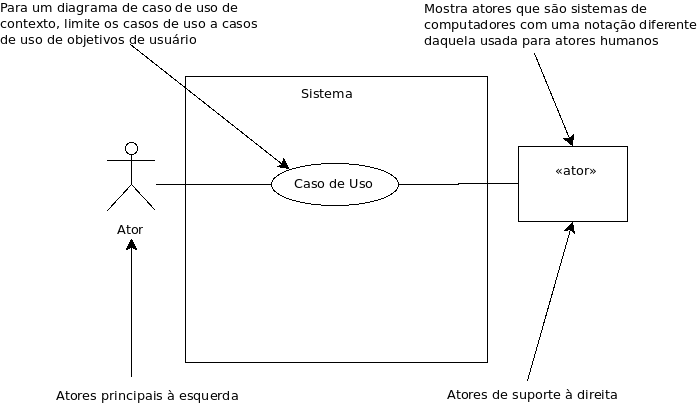
\includegraphics[scale=0.75]{images/exemplo-uml.png}
	\caption{Sugestões de notação de caso de uso proposto por ~\cite{larman08}}
	\label{fig:diagrama-uml}
\end{figure}

\subsubsection{Diagrama de Sequência}
O Diagrama de Sequência é um documento criado para ilustrar os eventos descritos em um caso de uso de forma sequencial e temporal, mostrando a interação de atores externos ao sistema e os eventos que eles geram durante essa interação. A UML possui uma notação específica para este diagrama, onde todos os elementos são representados.

Neste diagrama, são representados para cada cenário do caso de uso os eventos que os atores geram, bem como a ordem da sua interação. No diagrama os atores são representados na parte superior (com a mesma notação do diagrama de caso de uso). Abaixo dos atores é apresentada a linha de tempo, crescendo de cima para baixo. 

Durante a interação do ator com o sistema, eventos de sistema são gerados e iniciam toda a execução do cenário do caso de uso, ou operação do sistema. A execução dos eventos ocorre até o último evento cronológico na linha do tempo. Os eventos gerados pela interação entre os atores ocorrem na linha do tempo de forma cronológica e ordenada com a mesma ordem dos eventos do cenário do caso de uso.

A nomenclatura dos eventos deve sempre iniciar com um verbo, podendo ser seguida de um substantivo. Além disso, deve-se sempre expressar a nomenclatura em níveis genéricos verbais, nunca detalhando a funcionalidade do sistema.

A imagem~\ref{fig:exemplo-diagrama-sequencia} ilustra a notação de diagramas de sequência com todos os pontos que foram até agora expostos. Nela, é possível identificar a interação entre um ator e uma entidade do sistema. É fácil identificar que os eventos estão ocorrendo de forma ordenada de cima para baixo.
\begin{figure}
	\centering
	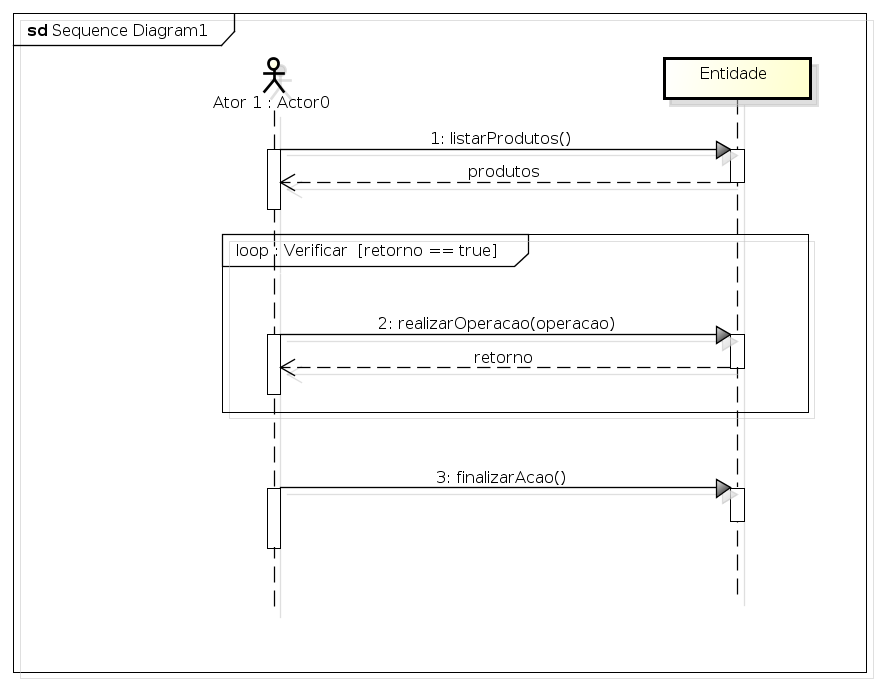
\includegraphics[scale=0.75]{images/exemplo-diagrama-sequencia.png}
	\caption{Notação de diagrama de sequência, exibindo a comunicação de um ator e uma entidade (sistema)}
	\label{fig:exemplo-diagrama-sequencia}
\end{figure}

O primeiro evento é iniciado pelo ator, onde o método~\emph(listarProdutos()) da Entidade é invocado. Esse método gera a resposta ~\emph(produtos) para o ator. A interação seguinte acontece dentro de um retângulo, do tipo~\emph{loop} e de nome "Verificar". Esse retângulo permite que o diagrama de sequências represente um loop, onde todos os eventos serão repetidos enquanto a condição de guarda for verdadeira, no caso do exemplo, enquanto retorno for igual a~\emph{true}. O UML permite diversos operadores além do loop, como por exemplo a negação, a assertiva, o~\emph{break}, dentre outros.

Dentro do retângulo, o ator chama o método~\emph(realizarOperacao), enviado o parâmetro~\emph{operação}. A entidade retorna um valor, que será testado na guarda para a continuidade da conversação. Por fim, o ator chama o método~\emph{finalizarAcao} da entidade. Por não haver outra interação em seguida, o cenário é considerado como encerrado. 

A importância do desenho de um diagrama de sequência está no fato de detalhar os eventos do sistema que são gerados pela interação de atores externos, pois assim é possível ter uma análise comportamental do sistema com base nesses eventos. Neste nível de análise, é possível estudar e projetar o comportamento do sistema no nível de projetar o que um sistema faz, porém sem necessariamente explicar como o faz~\ref{larman08}.

O diagrama de sequência geralmente está relacionado com o caso de uso, primeiramente pelo fato de descrever um cenário de caso de uso, mas também pelo fato de o caso de uso conter todos os detalhes do cenário. Ele apenas deixará claro a interação entre os atores e os eventos derivados dessa interação.

\section{Informática na Educação}

\section{Sistemas Multiagentes}

Este capítulo visa introduzir o conceito de sistemas multiagentes (SMA). Para tanto é necessário mostrar conceitos que são base para o entendimento de SMA, iniciando pela apresentanção alguns conceitos a cerca de Inteligencia Artificial (IA). Em seguida o trabalho disserta sobre a teoria relacionada à Agente, bem como suas arquiteturas. Só então são apresentados os conceitos de Sistemas Multiagentes (SMA), comunicação em um ambiente SMA e por fim a teoria sobre ontologias.

\subsection{Inteligência artificial}

De acordo com~\cite{poole98} identificamos que a definição de IA pode variar em duas dimensões principais. Usando a definição de sistemas computacionais que agem racionalmente temos:

\begin{quote}
\emph{Computational Intelligence is the study of the design of intelligent agents.}
\end{quote}

Nessa definição, é importante ressaltar que o agente é uma entidade que atua racionalmente, esperando-se que essa racionalidade e outras características o diferencie de simples programas.

Com o crescimento dos estudos relacionados a este campo a inteligência artificial ganhou várias áreas de atuação, permitindo assim a resolução de diversos desafios relacionados à aplicações modernas. Uma das áreas de atuação é o auxílio na execução de aplicações que resolvem problemas de alta complexidade. 

Atualmente várias aplicações podem exigir demais de~\emph{hardwares} mais modestos tornando inviável o tempo de execução daquela aplicação, sendo necessário um investimento maior e consequentemente encarecendo o seu valor. Dessa forma outras abordagems fazem-se necessárias, como a distribução da aplicação em vários computadores que dividem a sua execução. Este é o campo de estudo da Inteligência Artificial Distribuída: Sistemas que são compostos por vários agentes coletivos, ou seja, distribuem o trabalho uns com os outros. Cada agente pode possuir uma capacidade diferente, sendo possível realizar a tarefa de modo paralelo. 

\subsection{Agente}

De acordo com~\cite{novig95}, agentes são entidades (reais ou virtuais) que funcionam de forma autônoma em um ambiente, ou seja, não necessitam de intervenção humana para realizar processamento. Esse ambiente de funcionamento do agente geralmente contém vários outros agentes e é possível a comunicação entre eles através do ambiente por meio de troca de mensagens.

Em geral o funcionamento de agentes acontece de forma a perceberem o ambiente em que estão por meio de sensores, fazem análises com base nessa interação inicial e por fim podem agir sobre o ambiente de forma a modifica-lo por meio de efetuadores. A figura~\ref{fig:agente-basico} é uma ilustração do que foi dito.

\begin{figure}
	\centering
	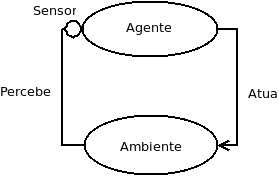
\includegraphics[scale=0.75]{images/agente-basico.png}
	\caption{Esquematização do funcionamento básico de um agente em um ambiente.}
	\label{fig:agente-basico}
\end{figure}

Alguns agentes seguem o princípio de racionalidade básico: sempre objetivam suas ações pela escolha da melhor ação possível segundo seus conhecimentos. Logo é possível inferir que a ação de um agente nem sempre alcança o máximo desempenho, sendo desempenho o parâmetro definido para medir o grau de sucesso da ação de um agente com base nos seus objetivos. São estes os chamados Agentes Racionais.

Como dito anteriormente, agentes estão presentes em um ambiente. O agente não tem controle total do ambiente, ele pode no máximo influenciá-lo com a sua atuação ou criar outros agentes. Podemos separar ambientes em classes: Software, Físico e Relidade virtual (simulação de ambientes reais em software). De acordo com~\cite{wooldridge04} temos, em geral, ambientes com propriedades inerentes à seu funcionamento:

\begin{itemize}
	\item Observável: Neste tipo de ambiente, os sensores dos agentes conseguem ter percepção completa do ambiente. Por exemplo, um sensor de movimento consegue ter visão total em um ambiente aberto.
	\item Determinística: O próximo estado do ambiente é sempre conhecido dado o estado atual do ambiente e as ações dos agentes. O oposto do ambiente determinístico é o estocástico, quando não temos certeza do estado do ambiente. Por exemplo, agentes dependentes de eventos climáticos.
	\item Episódico: A experiência do agente é dividida em episódios, onde cada episódio é a percepção do agente e a sua ação.
	\item Sequêncial: A ação tomada pelo agente pode afetar o estado do ambiente e ocasionar na mudança de estado
	\item Estático: O ambiente não é alterado enquanto um agente escolhe uma ação.
	\item Discreto: Existe um número definido de ações e percepções do agente para o ambiente em cada turno.
	\item Contínuo: As percepções e ações de um agente modificam-se em um espectro contínuo de valores. Por exemplo, temperatura de um sensor muda de forma contínua.
\end{itemize}

Na tabela~\ref{lista_agentes} mostramos alguns exemplos de agentes, apresentando as suas características já discutidas nesse trabalho.

\begin{table}
	\caption{Listagem de sistemas multiagentes com propriedades de medida de performance, ambiente, atuadores e sensores}
	\begin{tabular}{|p{3cm} | p{3cm} | p{2cm}| p{3cm} | p{3cm} |}
		\hline
		\textbf{Tipo de agente}	& \textbf{Medida de performance} & \textbf{Ambiente} & \textbf{Atuadores}  & \textbf{Sensores}	\\
		\hline
		Sensores de estacionamento	& Avarias no veículo & Carro e garagens & Freio do carro, controle de velocidade & Sensor de proximidade	\\
		\hline
		Jogos com oponente computador	& Quantidade de vitórias &	Software & Realizar jogada & Percepção do tabuleiro	\\
		\hline
		Agentes hospitalares		& Saúde do paciente & Paciente, ambiente médico & Diagnósticos & Entrada de sintomas do paciente	\\
		\hline
	\end{tabular}
	\label{lista_agentes}
\end{table}
 
A primeira linha da tabela~\ref{lista_agentes} apresenta um exemplo de agente atuando em um veículo como um sensor de estacionamento. Responsável por auxiliar o motorista no ato de estacionar o carro, o seu ambiente é da classe físico (considerando o carro e o ambiente onde está o carro). Seu sensor de proximidade é a percepção do ambiente e, caso detecte que está próximo de um obstáculo, pode atuar nos freios dos carros diminuindo a velocidade e evitando colisões. Avarias no carro podem indicar um mal funcionamento do sensor.

A segunda linha da tabela é apresentado o exemplo de agente atuando em um jogo avulso. Esse ambiente é dito dinâmico, pois a cada jogada de um oponente (real ou não), o agente deve analisar a jogada feita pelo seu oponente, irá calcular sua próxima jogada e a realizará. O objetivo principal do agente é a vitória. O ambiente que o agente atua é um software e o seu atuador é um algum mecanismo que permite que ele realize a jogada. O sensor é o mecanismo no qual o agente irá perceber a jogada realizada pelo oponente.

Por fim, a última linha da tabela~\ref{lista_agentes} expõe um exemplo de um agente médico atuando em um ambiente estático: Um paciente. Esse ambiente é classificado como estático por não ser alterado pelo agente nesse exemplo, porém é possível ser diferente em outras situações. O objetivo principal é monitorar a saúde do paciente, logo a medida de performance será a aproximação ou não do diagnóstico médico. Seu atuador não será diretamente no ambiente (corpo humano), será na forma de relatórios médicos e seus sensores podem variar de acordo com a doença a ser monitorada.

Conforme podemos encontrar em~\cite{wooldridge04}, podemos definir algumas noções gerais de agentes. A primeira, chamada de noção fraca, contém a maior parte dos agentes. Ela compreende os aspectos de \emph{reatividade}, \emph{proatividade} e \emph{habilidade social}. O conceito de reatividade  está ligado com o agente perceber o ambiente e reagir. Proatividade é a característica do agente tomar a iniciativa e agir sem a necessidade de nenhum estímulo. Habilidade social é a capacidade de interação com outros agentes.

Já a noção forte de agente envolve os seguintes aspectos: Mobilidade, veracidade, benevolência, racionalidade e cooperação. As definições são:
\begin{itemize}
	\item Mobilidade: O Agente deve pode mover-se no ambiente, por exemplo, em uma rede.
	\item Veracidade: Agente não comunica informações falsas.
	\item Benevolência: Agente ajudará os outros.
	\item Racionalidade: O agente não irá agir de forma a impedir a realização de seus objetivos.
	\item Cooperação: O agente coopera com o usuário.
\end{itemize}

\subsection{Arquitetura de agentes}

A arquitetura de agentes varia de acordo com a complexidade da sua autonomia, ou seja, com a capacidade de reagir aos estímulos do ambiente. Conforme verificado em~\cite{novig95}, os tipos de arquitetura são: orientadas à tabela, reflexiva simples, reflexiva baseado em modelo, baseada em objetivo, baseada em utilidade.

A primeira arquitetura a ser explorada é o agente orientado à tabelas. Todas as ações dos agentes dessa arquitetura são conhecidas e estão gravadas em uma tabela. Assim, quando o agente receber o estímulo ele já terá a ação a ser tomada previamente gravada em sua memória. Logo para construir esse tipo de agente, fica claro que além de saber todas percepções possívels, será necessário definir ações apropriadas para todas. Isso levará a tabelas muito complexas e o tamanho pode facilmente passar a ordem de milhões dependendo do número de entradas.

A arquitetura reflexiva simples é um dos tipos mais simples de agente. Nele, o agente seleciona a ação com base unicamente na percepção atual, desconsiderando assim uma grande tabela de decisões. A decisão é tomada com base de regras condição-ação: Se uma condição ocorrer, uma ação será tomada. Por exemplo, vamos supor um agente médico que determina o diagnóstico de uma doença no paciente caso exista alguma anomalia no organismo (Por exemplo, paciente com febre). Uma condição-ação poderia ser:

if anomalia-organismo then diagnóstico-médico

Esse tipo de agente é bastante simples, o que é uma vantagem comparado à arquitetura de tabela. Porém, essa abordagem requer um ambiente totalmente observável, visto que esse tipo de agente possui uma inteligência bastante limitada. No exemplo do agente médico existem diversas maneiras de se detectar uma anomalia no organismo do paciente, seria necessário conhecer todas as formas para usarmos uma abordagem reativa simples.

A arquitetura reflexiva baseada em modelos funciona de maneira similar a anterior. Nessa abordagem, é levado em conta a parte do ambiente que não é visível neste momento. E para saber o ``momento atual'' de um agente, é necessário guardar a informação de estado consigo. Para atualizar o estado do agente, é necessário conhecer como o mundo desenvolve-se independente do agente (no caso do exemplo, como o organismo funciona) e é necessário saber as ações dos agentes no ambiente. Esses dois conhecimentos do ambiente são chamados de \textbf{modelo do mundo}. O agente que usa esse tipo de abordagem é chamado de agente baseado em modelo.

Na arquitetura reflexiva baseada em objetivo, as ações do agente são tomadas apenas se o aproximam de alcançar um objetivo. Para isso, será necessário algo além do estado atual do ambiente: Será necessário informações do objetivo a ser atingido. Assim o agente pode combinar as informações do estado e o objetivo para determinar se deve ou não agir sobre o ambiente. Essa arquitetura porém é obviamente mais complexa e de certa forma ineficiente. Porém ela permite uma maior flexibilização das ações em determinados ambientes, visto que suas decisões são representadas de forma explícita e podem ser modificadas. É interessante notar que esse tipo de arquitetura não trata ações com objetivos conflitantes.

E por fim, a arquitetura reflexiva baseada em utilidade não utiliza apenas objetivos para realizar a próxima decisão, mas dá ao agente a capacidade de fazer comparações sobre o estado do ambiente e as ações a serem tomadas: Quais delas são mais baratas, confiáveis, baratas, rápidas do que as outras. A capacidade de avaliação do agente chama-se função de utilidade, que mapeia uma sequência de estados em um número real que determina o grau de utilidade. Esse mecanismo possibilita a decisão racional de escolha entre vários objetivos conflitantes. Por exemplo, escolher entre um objetivo mais barato ao invés de escolher entre o mais rápido.

\subsection{Sistemas Multiagentes}

Sistemas multiagentes são sistemas compostos por vários agentes capazes de se comunicar, possuindo uma linguagem de alto nível para isso. O agente deve ser conhecimento para realizar uma determinada tarefa e pode ou não cooperar com outros agentes para realizá-la.

Fica claro nessa definição que sistemas multiagentes

De acordo com~\cite{sarmento11}, podemos encontrar as seguintes características principais de ambientes em SMAs:
\begin{itemize}
	\item Ambientes SMAs fornecem protocolos específicos para comunicação e interação. Cada ambiente tem as suas particularidades: Alguns são em uma única máquina, outros são compartilhados com o mundo real e outros são distribuídos. Cabe a cada ambiente definir um protocolo onde todos agentes devem obedecer para comunicar-se.
	\item SMAs são tipicamente abertos.
	\item SMAs contém agentes que são autônomos e individualistas.
\end{itemize}

\subsection{Comunicação}

A comunicação é um dos aspectos mais importantes no desenvolvimento de SMAs. Problemas de sincronização entre as partes que se comunicam devem ser devidamente estudados. A situação mais simples possível da comunicação, onde o agente A envia uma mensagem ao agente B que está prontamente disponível para receber a mensagem nem sempre é a o cenário mais recorrente. Para tanto, é necessário entender os pormenores da comunicação em um Sistema Multiagente.

Em uma aplicação normal (Desktop ou Web), a comunicação entre objetos pode ser mais simplificada. Por exemplo, supondo uma aplicação em que existe dois objetos,~\emph{a} e~\emph{b} e que o objeto~\emph{a} tenha um método público chamado~\emph{m1}. O objeto~\emph{b} pode ser comunicar com o objeto~\emph{a} por meio do método~\emph{m1}, provavelmente da seguinte forma~\emph{a.m1(args)}, onde~\emph{args} são os argumentos enviados ao objeto~\emph{a} e a sintaxe pode ser diferente da apresentada, dependendo da linguagem de programação. É importante notar que o controle da execução do método~\emph{m1} não está no objeto~\emph{a}, mas sim no objeto~\emph{b}, que decide o momento o qual o método será invocado.

Esse cenário de comunicação é diferente em um ambiente SMA. Supondo dois agentes~\emph{a} e~\emph{b}, onde o agente~\emph{a} tem a capacidade de executar a ação $\alpha$. O agente~\emph{b} não poderá invocar diretamente o método que corresponde à ação $\alpha$, visto que os agentes são autônomos e independentes: Cada um tem somente tem total controle sobre suas ações e seus estados. O agente precisará enviar a solicitação da execução da ação $\alpha$ por meio de mensagem. Isso porém não garante que o agente~\emph{a} executará esta ação, pois pode não ser do seu interesse. Os agentes podem também influênciar o comportamento de outros agentes, alterando seu estado interno para a execução de ações e cooperando para o cumprimento do objetivo de outros agentes.

A comunicação dos agentes é baseada na teoria dos atos de fala (do inglês~\emph{Speech act theory}) e trata a comunicação como uma ação. A teoria dos atos de fala, publicada em 1962~\ref{austin62} por John Austin, onde ele percebe que certas expressões de linguagem natural, ou atos de fala, possuem a característica de realizar ação em um interlocutor, causando assim uma mudança de de estado da mesma forma que uma ação física. Logo, as expressões descrevem as ações por meio de desejos, habilidades e crenças.

De acordo com~\ref{verschueren09}, a teoria dos atos de fala possuem duas características:
\begin{itemize}
	\item A distinção entre um o significado expressado por uma expressão e a forma como essa expressão é utilizada.
	\item Expressões de todos os tipos podem ser considerados como atos, pois mudam o mundo de alguma forma.
\end{itemize}

Posteriormente o trabalho de John Searle~\ref{searle69}, relacionado ao de Austin, separa uma ação de um ato entre orador(~\emph{speaker}) e ouvinte(~\emph{hearer}) identifinca propriedades e conduções que um discurso deve conter para realizar ações sucedidas. Além disso, ele classifica alguns atos de discursos em 5 classes:
\begin{itemize}
	\item Representativas - Representa o ato de um orador representar uma verdade para o ouvinte. Pode ser entendido como uma ação de informar(~\emph{inform}).
	\item Diretivas - Tentativa do orador de fazer algum ouvinte realizar alguma ação por meio do seu ato.. Pode ser entendido como uma ação de requisição(~\emph{request}).
	\item Comissivas - O orador toma alguma atitude em relação à uma ação em andamento.
	\item Expressivas - Expressa algum estado psicológico.
	\item Declarações - Causa algum efeito relacionado a determinado assunto.
\end{itemize}

A comunicação então baseia-se nos atos de fala para prever a interação com seres humanos e é definida por meio de semânticas definidas pela teoria da Inteligência Artificial~\cite{wooldridge04}. O formalismo para a comunicação foi escolhido de forma que foi possível representar os atos de discursos em uma lógica multimodal, que contém os operadores de desejos, habilidades e crenças dos atos de discurso.

Da mesma forma que a teoria dos atos de fala influênciou na arquitetura da comunicação, ela influênciou também nas várias linguagens de comunicação dos agentes. Linguagens foram desenvolvidas para, não apenas representar ações de agentes, mas também para representar o conhecimento entre sistemas autônomos. No início dos anos 90, duas linguagens foram desenvolvidas pelo consórcio~\emph{Knowledge Sharing Effort}, encabeçados pela agência norte americana~\emph{Defense Advanced Research Projects Agency}(DARPA)~\cite{kse}.
\begin{itemize}
	\item ~\emph{Knowledge Query and Manipulation Language} (KQML) - Protocolo designado para a comunicação de agentes, em uma arquitetura que esses agentes sejam projetados para resolver problemas da arquitetura cliente-servidor~\cite{preece1997}. Não possui foco com o conteúdo da mensagem.
	\item \emph{Knowledge Interchange Format} (KIF) - Criada para facilitar a troca de conhecimento entre agentes, suas declarações são providas de significados que podem ser compreensíveis a qualquer agente que conheça a estrutura da linguagem. Não possui foco na transmissão da mensagem~\cite{kifmanual}.
\end{itemize}














